\providecommand{\main}{../..}
\documentclass[\main/thesis.tex]{subfiles}
\begin{document}

\section{The Maximum Numeral}\label{maximum}

A number is said to be the \textit{maximum} if there are no other numbers
greater than itself.
\scm{Hmm... I think the usual convention is that $m$ is {\em maximum} in
$S$ if $(\forall x \in S: x \leq m)$, and it is {\em maximal}
if $\neg (\exists x \in S: m \leq x)$. They differ when $(\leq)$ is not
a total order. I think you do mean maximum here, but the description
needs fixing?}
\begin{lstlisting}
Maximum : ∀ {b d o} → (xs : Numeral b d o) → Set
Maximum {b} {d} {o} xs = (ys : Numeral b d o) → ⟦ xs ⟧ ≥ ⟦ ys ⟧
\end{lstlisting}

If a numeral is a maximum
\footnote{More precisely, ``If a \text{value} of a numeral is a maximum ...''},
then its least significant digit (LSD) must be the greatest.

\begin{lstlisting}
Maximum⇒Greatest-LSD : ∀ {b} {d} {o}
    → (xs : Numeral b d o)
    → Maximum xs
    → Greatest (lsd xs)
\end{lstlisting}



\subsection{Properties of each Category}

\paragraph{NullBase}

\begin{center}
    \begin{adjustbox}{max width=\textwidth}
        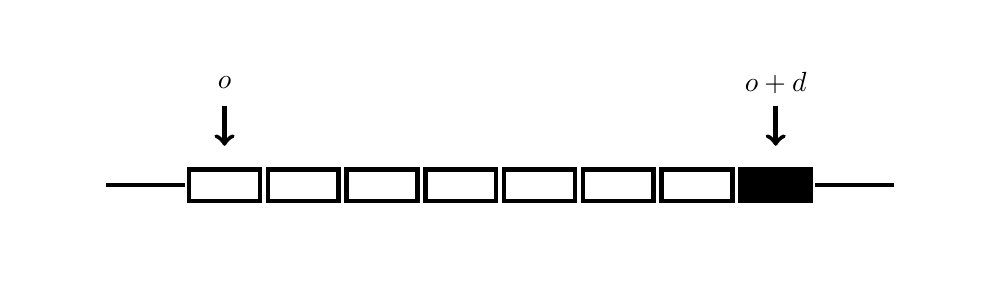
\begin{tikzpicture}
            % the frame
            \path[clip] (-1, -1) rectangle (11, 2);
            % the spine
            \draw[ultra thick] (0,0) -- (1,0);
            \draw[ultra thick] (9,0) -- (10,0);
            % the body

            \foreach \i in {1,...,7} {
                \draw[ultra thick, fill=white] ({\i+0.05}, -0.2) rectangle ({\i+0.95}, +0.2);
            };
            \draw[ultra thick, fill=black] ({8.05}, -0.2) rectangle ({8.95}, +0.2);

            % labels
            \draw[->, ultra thick] (1.5,1) -- (1.5,0.5)
                node at (1.5, 1.3) {$o$};
            \draw[->, ultra thick] (8.5,1) -- (8.5,0.5)
                node at (8.5, 1.3) {$o+d$};
        \end{tikzpicture}
    \end{adjustbox}
\end{center}

It is obvious that systems of {\lstinline|NullBase|} have \scmsubst{maxima}{maximum?}.
If a numeral's LSD happens to be the greatest,
then the numeral must be the maximum.

\begin{lstlisting}
Maximum-NullBase-Greatest : ∀ {d} {o}
    → (xs : Numeral 0 (suc d) o)
    → Greatest (lsd xs)
    → Maximum xs
\end{lstlisting}

With this lemma, we can tell whether a numeral is a maximum by looking at its
LSD. In case that the LSD is not the greatest, we could disprove the proposition
by contraposition.

\begin{lstlisting}
    Maximum-NullBase : ∀ {d} {o}
        → (xs : Numeral 0 (suc d) o)
        → Dec (Maximum xs)
    Maximum-NullBase xs with Greatest? (lsd xs)
    Maximum-NullBase xs | yes greatest =
        yes (Maximum-NullBase-Greatest xs greatest)
    Maximum-NullBase | no ¬greatest =
        no (contraposition (Maximum⇒Greatest-LSD xs) ¬greatest)
\end{lstlisting}

\paragraph{AllZeros}

\begin{center}
    \begin{adjustbox}{max width=\textwidth}
        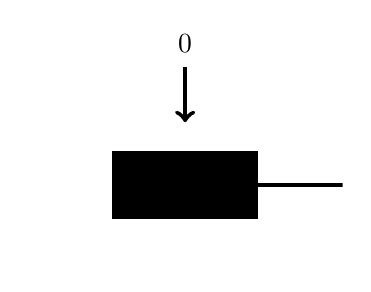
\begin{tikzpicture}
            % the frame
            \path[clip] (0, -1) rectangle (4, 2);
            % the spine
            \draw[ultra thick] (2,0) -- (4,0);
            % the body
            \draw[ultra thick, fill=black] ({1.1}, -0.4) rectangle ({2.9}, +0.4);

            % labels
            \draw[->, ultra thick] (2,1.5) -- (2,0.8)
                node at (2, 1.8) {$0$};
        \end{tikzpicture}
    \end{adjustbox}
\end{center}

\textit{All} numerals of systems of {\lstinline|AllZeros|} are maxima since they
are all mapped to $ 0 $.

\begin{lstlisting}
Maximum-AllZeros : ∀ {b}
    → (xs : Numeral b 1 0)
    → Maximum xs
Maximum-AllZeros xs ys = reflexive (
    begin
        ⟦ ys ⟧
    ≡⟨ toℕ-AllZeros ys ⟩
        zero
    ≡⟨ sym (toℕ-AllZeros xs) ⟩
        ⟦ xs ⟧
    ∎)
\end{lstlisting}

\paragraph{Proper}

On the contrary, there are no maxima in the systems of {\lstinline|Proper|}.
In fact, that is the reason why they are categorized as \textit{proper} in the
first place. The theorem below is proven by contradicting two propositions:

\begin{itemize}
    \item Given {\lstinline|claim : Maximum xs|}, we claim that {\lstinline|xs|}
        is greater than or equal to {\lstinline|greatest-digit d ∷ xs|},
        a numeral we composed by prefixing it with the greatest digit.
    \item On the other hand, we prove that {\lstinline|xs|} is less than
        {\lstinline|greatest-digit d ∷ xs|}.
\end{itemize}

\begin{lstlisting}
Maximum-Proper : ∀ {b d o}
    → (xs : Numeral (suc b) (suc d) o)
    → (proper : 2 ≤ suc (d + o))
    → ¬ (Maximum xs)
Maximum-Proper {b} {d} {o} xs proper claim = contradiction p ¬p
    where
        p : ⟦ xs ⟧ ≥ ⟦ greatest-digit d ∷ xs ⟧
        p = claim (greatest-digit d ∷ xs)
        ¬p : ⟦ xs ⟧ ≱ ⟦ greatest-digit d ∷ xs ⟧
        ¬p = <⇒≱ (
            start
                suc ⟦ xs ⟧
            ≈⟨ cong suc (sym (*-right-identity ⟦ xs ⟧)) ⟩
                suc (⟦ xs ⟧ * 1)
            ≤⟨ s≤s (n*-mono ⟦ xs ⟧ (s≤s z≤n)) ⟩
                suc (⟦ xs ⟧ * suc b)
            ≤⟨ +n-mono (⟦ xs ⟧ * suc b) (≤-pred proper) ⟩
                d + o + ⟦ xs ⟧ * suc b
            ≈⟨ cong
                (λ w → w + ⟦ xs ⟧ * suc b)
                (sym (greatest-digit-toℕ (Fin.fromℕ d)
                (greatest-digit-is-the-Greatest d)))
            ⟩
                ⟦ greatest-digit d ∷ xs ⟧
            □)
\end{lstlisting}

\subsection{Determine the Maximum}

We can \textit{decide} whether a numeral is a maximum by applying them to
lemmata of each category.

\begin{lstlisting}
Maximum? : ∀ {b d o}
    → (xs : Numeral b d o)
    → Dec (Maximum xs)
Maximum? {b} {d} {o} xs with numView b d o
Maximum? xs | NullBase d o = Maximum-NullBase xs
Maximum? xs | NoDigits b o = no (NoDigits-explode xs)
Maximum? xs | AllZeros b   = yes (Maximum-AllZeros xs)
Maximum? xs | Proper b d o proper = no (Maximum-Proper xs proper)
\end{lstlisting}

\paragraph{Summary}

\begin{center}
    \begin{adjustbox}{max width=\textwidth}
    \begin{tabular}{ | l | c | c | c | c | }
    \textbf{Properties} & \textbf{NullBase} & \textbf{NoDigits} & \textbf{AllZeros} & \textbf{Proper} \\
    \hline
    has an maximum & yes & no & yes & no \\
    \end{tabular}
    \end{adjustbox}
\end{center}

\end{document}
